\lecturechapter{Friday}{Feb 20th}{February 20th 2026}{Topology of Metric Spaces: Open and Closed Sets}

\begin{nice-box}[Context]
This lecture marks the transition from the basic definitions of metric spaces to the study of their \emph{topology}. The lecturer, Joaquim Serra, reviews the concepts of convergence and completeness before introducing the fundamental building blocks of topological spaces: open and closed sets. The discussion emphasizes the use of axioms to prove properties that will later be applied to multivariable differentiation and integration.
\end{nice-box}

% ==========================================
% SECTION 1: REVIEW AND INTRODUCTION
% ==========================================
\section{Review of Previous Lectures}

\begin{spoken-clean}[00:00:00 - 00:01:51]
We can continue. Uh, good afternoon. We can --- we can continue where we left it last time. So, I remind --- so just a quick summary of what we saw the last lectures. First lecture was mostly introduction, but then we saw metric spaces. And I told you --- because people already asked me, even though I thought the first day --- why we studied metric spaces. So, the model --- whenever it gets too abstract, the model you need to have in mind all the time for this $(X, d)$ metric space is $\mathbb{R}^n$ with the Euclidean distance, okay? So, whenever you have doubts, just plug $\mathbb{R}^n$ where there is an $X$ (a capital $X$) and $d$ is the usual --- the modulus of the difference of the points. And, um, I said that I wanted to do this in this more general framework because later, in the last part of the course, we will use other spaces. Okay?
\end{spoken-clean}

\begin{math-stroke}[Summary of Metric Space Foundations]
\begin{ai-type-check-invisible-content}
% (X, d) is a metric space.
% x_n is a sequence in X.
\end{ai-type-check-invisible-content}
The core structure studied thus far is the metric space $(X, d)$.
\begin{itemize}
    \item \textbf{Standard Model:} $(\mathbb{R}^n, d_{\text{Eucl}})$, where $d(x, y) = \|x - y\|$.
    \item \textbf{Sequences:} $(x_n)_{n \ge 0} \subset X$ converges to $x \in X$ ($x_n \to x$) if $d(x_n, x) \to 0$.
    \item \textbf{Completeness:} A space is \emph{complete} if every Cauchy sequence converges. We proved that $\mathbb{R}^n$ is a complete metric space.
\end{itemize}
\end{math-stroke}

\begin{spoken-clean}[00:01:51 - 00:02:22]
And for good reason. It's not --- I mean, we will use to prove some theorems in the --- in the course, the space of continuous functions. Uh, but --- if you want for the --- this is not something that belongs to mathematicians, right? Let me say very quickly for the physicists: so in classical mechanics, the points in the space is a vector in $\mathbb{R}^n$, right? But when you --- you will go to quantum mechanics, what is a point? What is the position of a particle in space? Is the wave function. This is a function. So, the function --- the wave functions are naturally points in your space, right? So, this is what we are saying here. We are trying to say things more general to be able to understand, um, the things that come naturally in the physics, for instance.
\end{spoken-clean}

\begin{didactic-insight}[The Physical Motivation for Abstraction]
The lecturer provides a profound justification for studying abstract metric spaces. In classical mechanics, a "point" is a coordinate in $\mathbb{R}^n$. In quantum mechanics, a "state" is a wave function. By treating functions as points in a metric space, the tools of Analysis (limits, continuity, topology) become directly applicable to the most advanced models of physics.
\end{didactic-insight}

\begin{spoken-clean}[00:02:22 - 00:03:13]
Okay. So, now, in this framework of metric spaces, we saw what it means a sequence, what it means that a sequence converges, what is a Cauchy sequence, what is a complete metric space, and we proved that $\mathbb{R}^n$ is always a complete metric space using that $\mathbb{R}$ is complete. This last time. And today we will see, uh, what is the definition of open and closed sets in a metric space and the notion of continuous functions in the setup of metric spaces. So, let me start with the definition of open set. So, let me start maybe with the definition of open ball. Open ball.
\end{spoken-clean}

% ==========================================
% SECTION 2: TOPOLOGY OF METRIC SPACES
% ==========================================
\setcounter{section}{1}
\section{Topology of Metric Spaces}
\subsection{Open and Closed Sets}

\begin{math-stroke}[Definition: Open Ball]
\setcounter{theorem}{37}
\begin{definition}[Open Ball]\label{def:open-ball}
We define the \emph{open ball} of radius $r > 0$ centered at a point $x \in X$ in a metric space $(X, d)$ as:
\[ B(x, r) = \{ y \in X \mid d(y, x) < r \} \]
\end{definition}

\begin{explanation-of-steps}
The open ball is the set of all points whose distance to the center $x$ is strictly less than the radius $r$. The strict inequality ($<$) is what makes the ball \qt{open}—it does not include its boundary.
\end{explanation-of-steps}

\begin{nice-box}[Notation Note]
The lecturer notes that $B_r(x)$ is an equivalent and common notation for $B(x, r)$ found in many textbooks.
\end{nice-box}
\end{math-stroke}

\begin{spoken-clean}[00:03:13 - 00:05:12]
So, we --- we define --- define the open ball, open ball of radius $r$ positive centered at a given point $x$ in my metric space as --- and we will denote with this: is ball centered at $x$ with radius $r$. Sometimes you will see equivalent notation is the ball of radius $r$ centered at $x$. This is also in many notes and books. Is the same. Okay? This is by definition the set of points in my space such that the distance --- sorry, the points will be $y$ --- such that the distance between $y$ and $x$ is less than $r$, right?

So, if you want a drawing of that, in the Euclidean space --- in a --- in a general metric space I cannot draw anything because it's too general --- but in the Euclidean space, let's say in $\mathbb{R}^2$, the metric ball would be the ball. So, the --- the open ball would be this, right? \inlinemetanote{Draws a circle on the board} What is inside of the --- of the ball. And it's open because you don't include --- if you want I can --- I can put the boundary of the ball, that we will introduce in a --- today also in a --- in a general topological space what the boundary means. This surface of the ball is not included, because there is a strict inequality, okay? The points that are at exactly distance $r$, I don't take them. This is the open ball.
\end{spoken-clean}

\begin{math-stroke}[Visualizing the Open Ball in \texorpdfstring{$\mathbb{R}^2$}{R2}]
\begin{center}
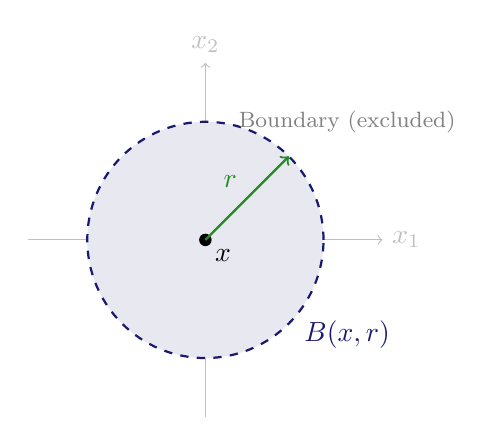
\begin{tikzpicture}[scale=1.5]
% \begin{ai-tikz-planner-invisible-content}
% 1. Background: 2D Axes.
% 2. Midground: A dashed circle representing the boundary.
% 3. Foreground: Shaded interior and center point x.
% \end{ai-tikz-planner-invisible-content}
    % Axes
    \draw[->, gray!50] (-1.5,0) -- (1.5,0) node[right] {$x_1$};
    \draw[->, gray!50] (0,-1.5) -- (0,1.5) node[above] {$x_2$};

    % The Ball
    \draw[dashed, thick, MidnightBlue, fill=MidnightBlue!10] (0,0) circle (1cm);
    \fill (0,0) circle (1.5pt) node[below right] {$x$};
    \draw[->, thick, ForestGreen] (0,0) -- (0.707, 0.707) node[midway, above left] {$r$};
    
    \node[MidnightBlue] at (1.2, -0.8) {$B(x, r)$};
    \node[gray, font=\footnotesize] at (1.2, 1.0) {Boundary (excluded)};
\end{tikzpicture}
\end{center}
\end{math-stroke}

\begin{spoken-clean}[00:05:12 - 00:06:15]
Now, next definition is open and closed sets. So, we say that a set $U$ of my metric space $X$ is open if for every $x$ in $U$, exists some positive radius $r$ (depending on $x$, possibly) such that the ball of radius $r$ centered at $x$ is contained in $U$. So, I will draw some in $\mathbb{R}^2$ some open set. Is essentially any --- any set --- this is a bit --- heuristically, this is the idea, right? Then we will see concrete open sets. But is a set that does not include its contour. So, its boundary. Again, I --- I didn't define the boundary yet, but now you know --- you --- you have some common sense knowledge of what is a boundary of this set, that is this part --- is the skin of the set, right? If the set is the inside without the skin, this is open.
\end{spoken-clean}

\begin{math-stroke}[Definition: Open and Closed Sets]
\setcounter{theorem}{38}
\begin{definition}[Open Set]\label{def:open-set}
A subset $U \subseteq X$ of a metric space $(X, d)$ is \emph{open} if every point in $U$ is the center of some open ball entirely contained within $U$:
\[ \forall x \in U, \exists r > 0 \text{ s.t. } B(x, r) \subseteq U \]
\end{definition}

\begin{center}
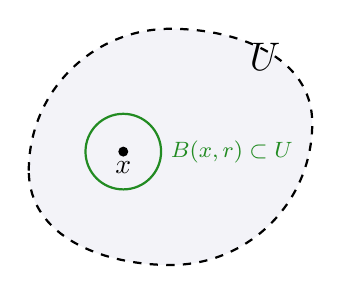
\begin{tikzpicture}[scale=1.2]
% \begin{ai-tikz-planner-invisible-content}
% 1. Background: A generic "potato" shape with a dashed boundary.
% 2. Midground: A point x inside.
% 3. Foreground: A small solid circle around x representing B(x, r).
% \end{ai-tikz-planner-invisible-content}
    % The Open Set U
    \draw[dashed, thick, fill=MidnightBlue!5] 
        (0,0) to[out=90,in=180] (1.5,1.5) 
        to[out=0,in=90] (3,0.5) 
        to[out=-90,in=0] (1.5,-1) 
        to[out=180,in=-90] cycle;
    \node at (2.5, 1.2) {\Large $U$};

    % Point x and its ball
    \coordinate (X) at (1, 0.2);
    \fill (X) circle (1.5pt) node[below] {$x$};
    \draw[thick, ForestGreen] (X) circle (0.4cm);
    \node[ForestGreen, right] at (1.4, 0.2) {\footnotesize $B(x, r) \subset U$};
\end{tikzpicture}
\end{center}

\begin{explanation-of-steps}
The intuition behind an open set is that no point in the set is on the \qt{edge}. For any point $x$, you can always move a tiny distance in any direction and still remain inside the set.
\end{explanation-of-steps}
\end{math-stroke}

% \begin{ai-global-state-checkpoint-invisible-content}
% timestamp: 00:06:00
% topic: Definitions of open balls and open sets.
% board_state: def:open-ball, def:open-set
% next_goal: Provide a concrete example of an open set (the square).
% open_loops: none
% \end{ai-global-state-checkpoint-invisible-content}

\begin{spoken-clean}[00:06:15 - 00:08:37]
Why? Because any point here, you can take a ball --- depending on the distance to the boundary, right? Depending on the distance to the skin. You make the ball super small and it will be contained in the set. Is --- as I said, any point in the interior will be at positive distance from the skin.

So, if you want a more concrete example, take the set $(0, 1) \times (0, 1)$, the square, open square, subset $\mathbb{R}^2$. This --- prove that it is open. Exercise. So, you take this square... \inlinemetanote{Draws a dashed square on the board} You take a point here. A point in the square will have two coordinates. And now, what is the definition of open? If you take the point --- this point is $(x_1, x_2)$ --- you need to find a --- you need to construct a radius $r$ positive such that the whole ball centered at this given point belongs to the --- to the square. In the case of the square, what is the formula for the radius? Well, you can take $r$ equal, I don't know, something like the minimum between this distance, this distance, this distance, and this distance. So, it will be something like the minimum between $x_1, x_2, 1 - x_1$ and $1 - x_2$. You can check that this radius works. The minimum of these four numbers. Right?
\end{spoken-clean}

\begin{math-stroke}[Example: The Open Unit Square]
Consider the open unit square in $\mathbb{R}^2$:
\[ U = (0, 1) \times (0, 1) \subset \mathbb{R}^2 \]
\begin{center}
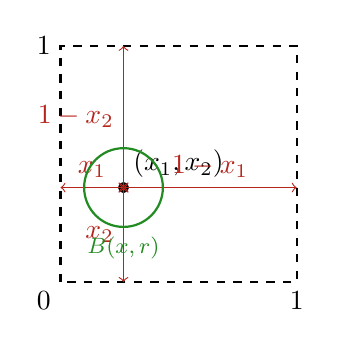
\begin{tikzpicture}[scale=2]
% \begin{ai-tikz-planner-invisible-content}
% 1. Background: Dashed square boundary.
% 2. Midground: Point x = (x1, x2).
% 3. Foreground: Arrows showing distances to the four boundaries.
% \end{ai-tikz-planner-invisible-content}
    % The Square
    \draw[dashed, thick] (0,0) rectangle (1.5, 1.5);
    \node[below left] at (0,0) {$0$};
    \node[below] at (1.5, 0) {$1$};
    \node[left] at (0, 1.5) {$1$};

    % Point x
    \coordinate (X) at (0.4, 0.6);
    \fill (X) circle (1pt) node[above right] {$(x_1, x_2)$};

    % Distances to boundaries
    \draw[<->, BrickRed, thin] (0.4, 0) -- (0.4, 0.6) node[midway, left] {$x_2$};
    \draw[<->, BrickRed, thin] (0, 0.6) -- (0.4, 0.6) node[midway, above] {$x_1$};
    \draw[<->, BrickRed, thin] (0.4, 0.6) -- (0.4, 1.5) node[midway, left] {$1-x_2$};
    \draw[<->, BrickRed, thin] (0.4, 0.6) -- (1.5, 0.6) node[midway, above] {$1-x_1$};
    
    % The Ball
    \draw[ForestGreen, thick] (X) circle (0.25cm);
    \node[ForestGreen, below] at (0.4, 0.35) {\footnotesize $B(x, r)$};
\end{tikzpicture}
\end{center}
\begin{explanation-of-steps}
To prove $U$ is open, for any $(x_1, x_2) \in U$, we must find $r > 0$ such that $B(x, r) \subset U$. The distance to the nearest boundary is given by:
\[ r = \min(x_1, x_2, 1 - x_1, 1 - x_2) \]
Since $0 < x_1, x_2 < 1$, all four terms are strictly positive, so $r > 0$. Any point $y$ within distance $r$ of $x$ will necessarily have coordinates between $0$ and $1$, remaining inside the square.
\end{explanation-of-steps}
\end{math-stroke}

\begin{spoken-clean}[00:08:37 - 00:10:16]
Okay. Second point in the definition is what is a closed set. So, $A$ subset $X$ is called closed if the complement is open. $X - A$ is open. This set $(0, 1) \times (0, 1)$ is not closed. You can show. Instead, this set --- for instance, $[0, 1] \times [0, 1]$ --- this set is closed. Now it needs to contains the skin to be closed. Because then, when you pass to the open --- to the complement that is by definition open, it need not to contain the boundary, right? So, the closed sets, we draw them with their skin. This is closed. $A$.
\end{spoken-clean}

\begin{math-stroke}[Definition: Closed Set]
\begin{definition}[Closed Set]\label{def:closed-set}
A subset $A \subseteq X$ is \emph{closed} if its complement in $X$ is an open set:
\[ A \text{ is closed} \iff X \setminus A \text{ is open} \]
\end{definition}

\begin{center}
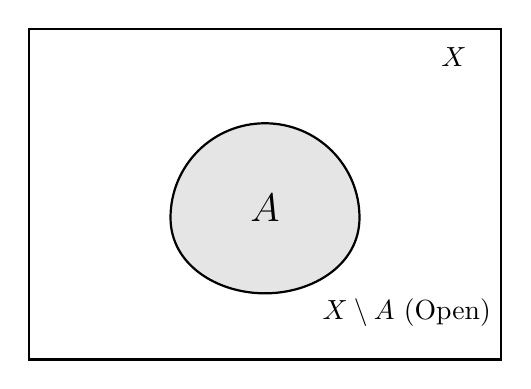
\begin{tikzpicture}[scale=1.2]
% \begin{ai-tikz-planner-invisible-content}
% 1. Background: A solid bounding box representing X.
% 2. Midground: A solid "potato" shape representing A.
% 3. Foreground: Labels for A and X \ A.
% \end{ai-tikz-planner-invisible-content}
    % Ambient Space X
    \draw[thick] (-1,-1.5) rectangle (4, 2);
    \node at (3.5, 1.7) {$X$};

    % Closed Set A
    \draw[thick, fill=gray!20] 
        (0.5,0) to[out=90,in=180] (1.5,1) 
        to[out=0,in=90] (2.5,0) 
        to[out=-90,in=0] (1.5,-0.8) 
        to[out=180,in=-90] cycle;
    \node at (1.5, 0.1) {\Large $A$};
    
    \node at (3, -1) {$X \setminus A$ (Open)};
\end{tikzpicture}
\end{center}

\begin{explanation-of-steps}
A closed set \qt{contains its boundary}. For example, the closed unit square $[0, 1] \times [0, 1]$ is closed because its complement (everything outside the square) is an open set.
\end{explanation-of-steps}
\end{math-stroke}

\begin{spoken-clean}[00:10:16 - 00:12:03]
Okay. And maybe the last part of this definition that you will not use --- we will not use actually --- but --- but is something that is a --- a common term that you will find in books and it's good that you know, is what is the topology. So, you will see in the notes you will see the word topology many times. You are not yet studying topology but --- just for information, the word topology --- topology generated --- so the --- the topology associated to the distance $d$ is the --- we can put a $\mathcal{T}$ like this, a sort of calligraphic $\mathcal{T}$, is the collection of all the open sets. This is the topology. So, when we --- when we say that something is a topological notion, it has to do with this collection of open sets.
\end{spoken-clean}

\begin{math-stroke}[Definition: Topology]
\begin{definition}[Topology]\label{def:topology}
The \emph{topology} $\mathcal{T}$ on a metric space $(X, d)$ is the collection of all open subsets of $X$:
\[ \mathcal{T} = \{ U \subseteq X \mid U \text{ is open} \} \]
\end{definition}
\end{math-stroke}

% \begin{ai-global-state-checkpoint-invisible-content}
% timestamp: 00:12:00
% topic: Definitions of closed sets and topology.
% board_state: def:closed-set, def:topology
% next_goal: State and prove the lemma on unions and intersections of open sets.
% open_loops: none
% \end{ai-global-state-checkpoint-invisible-content}

\begin{spoken-clean}[00:12:03 - 00:13:41]
Now, to see a bit more what are --- because this is still a bit abstract --- to see a bit more practically how we identify open and closed sets, uh, we are going to do it through sequences. Okay? So, this is the... well, let me first do a lemma, maybe, that it we will use many times. Lemma: unions and intersections of open sets. This is one of the basic properties. It's --- it's very simple, but since we will use many, many times, I prove it now. So, it says that --- I will put it with words and then we will prove with symbols. So, arbitrary unions of open sets are open.
\end{spoken-clean}

\begin{nice-box}[Proposition: Unions and Intersections of Open Sets]
\setcounter{theorem}{42}
\begin{proposition}\label{prop:open-sets-unions-intersections}
In any metric space $(X, d)$:
\begin{enumerate}
    \setcounter{enumi}{0} \item The union of an \emph{arbitrary} collection of open sets is open.
    \setcounter{enumi}{1} \item The intersection of a \emph{finite} collection of open sets is open.
\end{enumerate}
\end{proposition}
\end{nice-box}

\begin{spoken-clean}[00:13:41 - 00:15:50]
So, this means that if you have some collection $\{U_i\}_{i \in I}$ of $U_i$ subset $X$ open, then the union of this collection (that can be --- the union of the collection is also open). Right? And also finite intersections of open sets are open. Right? So, this means that if $I$ is finite (is a finite set), the intersection --- let's say, let's put it like this: the intersection of $U_i$ for $i$ between $1$ and capital $N$ (a bounded number) --- this is open set.
\end{spoken-clean}

\begin{proof}[Proof of Proposition \ref{prop:open-sets-unions-intersections}]
\begin{spoken-clean}[continued]
The proof of this is just using the definition. So, if I want to check that a union is open, I take a point $x$ in this set that is the union. Let me call this in the union. And then this in particular $x$ belongs to one of them, because it's a union. I call $i_0$ is one of the $i$s. I any of them. And then since this --- this guy is open, exists some radius such that the ball of radius $r$ centered at $x$ is contained in $U_{i_0}$. But this is contained in the union. Which proves that this union is open, right?
\end{spoken-clean}

\begin{math-stroke}[Proof: Arbitrary Unions]
Let $\{U_i\}_{i \in I}$ be a collection of open sets. Let $x \in \bigcup_{i \in I} U_i$.
\begin{description}
    \item[Step 1:] By the definition of union, there exists some index $i_0 \in I$ such that $x \in U_{i_0}$.
    \item[Step 2:] Since $U_{i_0}$ is open, there exists $r > 0$ such that $B(x, r) \subseteq U_{i_0}$.
    \item[Step 3:] Since $U_{i_0} \subseteq \bigcup_{i \in I} U_i$, it follows that $B(x, r) \subseteq \bigcup_{i \in I} U_i$.
\end{description}
Thus, the union is open.
\end{math-stroke}

\begin{spoken-clean}[continued]
With the finite intersection, you can do as an exercise. But I will tell you how to do, okay? Now explain the proof with, yeah. \inlinemetanote{The lecturer retrieves the catch-box microphone}
\end{spoken-clean}

\begin{student-interaction}[Student Question]
Except for the empty set and the set $X$ itself, can you give us some examples of both closed and open sets?
\end{student-interaction}

\begin{spoken-clean}[continued]
Um, we will discuss this when we --- when we discuss connected spaces. Okay? This is a good question. So, the --- the whole space and the empty set are always open and closed, and I will emphasize this when we see connected spaces. So, you need to wait a bit more. I could give an example, but it's not very interesting. It's just a disconnected space like the --- the union, the disjoint union of two intervals or something like that, then each interval is open and closed. But this will not be very interesting. You will see the interest of this question when we see connected spaces. Okay? But --- is a fair question.
\end{spoken-clean}

\begin{math-stroke}[Proof: Finite Intersections]
\begin{ai-proof-skeleton-invisible-content}
% 1. Take x in the intersection of U_1, ..., U_N.
% 2. x is in each U_i, so there exists r_i such that B(x, r_i) is in U_i.
% 3. Take r = min(r_1, ..., r_N).
% 4. Then B(x, r) is in every U_i, so it's in the intersection.
\end{ai-proof-skeleton-invisible-content}
Let $U_1, \dots, U_N$ be open sets. Let $x \in \bigcap_{i=1}^N U_i$.
\begin{description}
    \item[Step 1:] Since $x$ is in the intersection, $x \in U_i$ for all $i \in \{1, \dots, N\}$.
    \item[Step 2:] Since each $U_i$ is open, for each $i$ there exists $r_i > 0$ such that $B(x, r_i) \subseteq U_i$.
    \item[Step 3:] Let $r = \min(r_1, r_2, \dots, r_N)$. Since we are taking the minimum of a \emph{finite} number of positive values, $r > 0$.
    \item[Step 4:] For this $r$, $B(x, r) \subseteq B(x, r_i) \subseteq U_i$ for all $i$. Therefore, $B(x, r) \subseteq \bigcap_{i=1}^N U_i$.
\end{description}
Thus, the finite intersection is open.
\end{math-stroke}
\end{proof}

% \begin{ai-global-state-checkpoint-invisible-content}
% timestamp: 00:18:00
% topic: Unions and intersections of open sets.
% board_state: prop:open-sets-unions-intersections, proof:unions-open
% next_goal: State and prove the lemma for closed sets using De Morgan's laws.
% open_loops: none
% \end{ai-global-state-checkpoint-invisible-content}

\begin{spoken-clean}[00:18:05 - 00:19:05]
So, I am saying that when --- when you take open sets, when you take finitely many intersections of open sets, uh, you get something open. Why? I will say with words, and then you try to write down, okay? So, you --- you have finitely many open sets. And now you take a point that is in the intersection of these finitely many. Right? This means that the point is in all of them. And now, for each of the sets, you pick a radius that is different in every time, but there are finitely many radii that you can put your ball in the open set. And if you take the minimum of all these radii, it will be good. With the minimum of the finitely many radii, you will fall inside of the intersection. Okay?
\end{spoken-clean}

\begin{spoken-clean}[00:19:05 - 00:21:42]
You don't need to understand what I said, please try to do the exercise. If there are problems doing this, uh, you have it in the notes. But I think this is a --- is very good to try in these first proofs of the --- of the theory that are very short one-line proofs, is very good opportunity to do as an exercise to see if we understood the definitions. Because is one line. So, it's not --- you don't need to think too much.

Okay. Now, analogous lemma but for closed sets. Unions and intersections of closed sets. And it is the same but --- the same but the opposite. So, it says that finite unions of closed sets are closed, and arbitrary intersections of closed sets are closed. And the proof is essentially --- well, you can repeat the same proof or you can reason a bit more --- or a variant of the same proof --- or you can reason passing to the complement. So, you can use that when you have a finite union --- so remember that being closed is defined as the complement being open. So, if you pass to the complement, the complementation converts closed sets in open and open in closed, right? So, you can always pass statements about open sets to the complement and you get a statement about closed sets. If you have some property of open sets and you pass to the complements (all the statement), you get a property of closed sets. And this is what we have here. Why? Because $X$ minus a union of sets is the same as the intersection of the complements, right?
\end{spoken-clean}

\begin{nice-box}[Proposition: Unions and Intersections of Closed Sets]
\setcounter{theorem}{43}
\begin{proposition}\label{prop:closed-sets-unions-intersections}
In any metric space $(X, d)$:
\begin{enumerate}
    \setcounter{enumi}{0} \item The intersection of an \emph{arbitrary} collection of closed sets is closed.
    \setcounter{enumi}{1} \item The union of a \emph{finite} collection of closed sets is closed.
\end{enumerate}
\end{proposition}
\end{nice-box}

\begin{math-stroke}[Proof via De Morgan's Laws]
\begin{proof}
The properties of closed sets follow directly from the properties of open sets using De Morgan's Laws:
\begin{align}
X \setminus \left( \bigcup_{i \in I} A_i \right) &= \bigcap_{i \in I} (X \setminus A_i) \label{eq:demorgan-union} \\
X \setminus \left( \bigcap_{i \in I} A_i \right) &= \bigcup_{i \in I} (X \setminus A_i) \label{eq:demorgan-intersection}
\end{align}
\begin{description}
    \item[Arbitrary Intersections:] Let $\{A_i\}_{i \in I}$ be closed. Then each $X \setminus A_i$ is open. By Proposition \ref{prop:open-sets-unions-intersections}, their arbitrary union $\bigcup (X \setminus A_i)$ is open. By Equation \ref{eq:demorgan-intersection}, this union is the complement of the intersection $\bigcap A_i$. Since the complement is open, the intersection is closed.
    \item[Finite Unions:] Let $A_1, \dots, A_N$ be closed. Then each $X \setminus A_i$ is open. By Proposition \ref{prop:open-sets-unions-intersections}, their finite intersection $\bigcap (X \setminus A_i)$ is open. By Equation \ref{eq:demorgan-union}, this intersection is the complement of the union $\bigcup A_i$. Since the complement is open, the union is closed.
\end{description}
\end{proof}
\end{math-stroke}

\begin{spoken-clean}[00:21:42 - 00:24:23]
So, when you do the complement of a union, you get the intersection of the complements. And the same: the complement of a intersection is equal to the union of the complements. And then you apply the previous result. Because if these sets are closed, these sets will be open. And the intersection --- so the finite intersection of open is open. Okay?

Let me give some example very --- very easy that this property --- when we said finite intersections or finite unions --- is important that it is finite. That when you get infinite intersections of open sets, you can get a closed set that is not open. Example: finite is important. So, if you take the simplest possible --- well, the simplest possible no, but one of the spaces that you are most familiar with that is $\mathbb{R}$ with the distance of the absolute value (with the Euclidean distance), and you take the sets $U_k = (-1/k, 1/k)$. And you take its intersection, then the intersection for $k$ equals $1$ to infinity of $U_k$ --- this gives you the point $\{0\}$. So, these are open intervals, and it's very easy because the intervals do not contain the end points, each of them is open. But when you do their intersection, you get just the point zero, and the point zero is not open because is --- you cannot put any ball in that contains anything, right? The point zero is closed but is not open. So, these are open and this is not open! That's why it's important that the intersection is finitely many.
\end{spoken-clean}

\begin{math-stroke}[Example: Infinite Intersection of Open Sets]
\setcounter{theorem}{44}
\begin{example}\label{ex:infinite-intersection-open}
The finiteness condition in Proposition \ref{prop:open-sets-unions-intersections} is necessary. Consider the collection of open intervals in $\mathbb{R}$:
\[ U_k = \left( -\frac{1}{k}, \frac{1}{k} \right) \quad \text{for } k \in \mathbb{N} \]
The intersection of this infinite collection is:
\[ \bigcap_{k=1}^\infty U_k = \{ 0 \} \]
\begin{center}
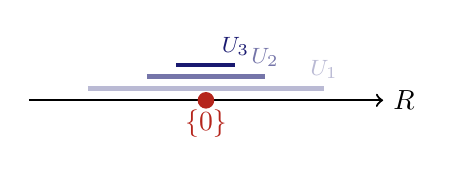
\begin{tikzpicture}[scale=1.5]
% \begin{ai-tikz-planner-invisible-content}
% 1. Background: Horizontal axis.
% 2. Midground: Nested intervals (-1, 1), (-1/2, 1/2), etc.
% 3. Foreground: The point {0} at the center.
% \end{ai-tikz-planner-invisible-content}
    \draw[->, thick] (-1.5,0) -- (1.5,0) node[right] {$\mathbb{R}$};
    
    % Intervals
    \draw[ultra thick, MidnightBlue!30] (-1, 0.1) -- (1, 0.1);
    \node[MidnightBlue!30, above] at (1, 0.1) {\footnotesize $U_1$};
    
    \draw[ultra thick, MidnightBlue!60] (-0.5, 0.2) -- (0.5, 0.2);
    \node[MidnightBlue!60, above] at (0.5, 0.2) {\footnotesize $U_2$};
    
    \draw[ultra thick, MidnightBlue] (-0.25, 0.3) -- (0.25, 0.3);
    \node[MidnightBlue, above] at (0.25, 0.3) {\footnotesize $U_3$};

    % The limit point
    \fill[BrickRed] (0,0) circle (2pt) node[below] {$\{0\}$};
\end{tikzpicture}
\end{center}
\begin{explanation-of-steps}
While each $U_k$ is an open set, their infinite intersection is the singleton set $\{0\}$, which is \emph{closed} but \emph{not open} in $\mathbb{R}$. This demonstrates that the property of openness is not necessarily preserved under infinite intersections.
\end{explanation-of-steps}
\end{example}
\end{math-stroke}

% \begin{ai-global-state-checkpoint-invisible-content}
% timestamp: 00:24:00
% topic: Counter-example for infinite intersections of open sets.
% board_state: ex:infinite-intersection-open
% next_goal: Define interior and closure.
% open_loops: none
% \end{ai-global-state-checkpoint-invisible-content}

\begin{spoken-clean}[00:24:23 - 00:27:06]
Okay. So, now we will define something interesting that is what we were saying there heuristically. So, what is the interior and the boundary of a set in a metric space. So, given a set --- let me call the set $\Omega$ subset $X$ --- $(X, d)$ is a metric space. I define the interior of $\Omega$. This is called the interior. Maybe I will not put parenthesis. I will say $\operatorname{int} \Omega$ or sometimes you put $\Omega$ with a point like this, or with a point here, depends on the source. The interior --- this is what is called the interior of $\Omega$. This is by definition the largest open set contained in $\Omega$. So, you have your set $\Omega$ and you look at all the open sets that are contained and you get the largest one is the union of all the open sets that contain $\Omega$. So, is the union of the $U$ subset $\Omega$ such that $U$ is open. Right? This is the interior.

Now, I also define the closure that you know from $\mathbb{R}$, right? The closure of some set is the set of points $x$ in $X$ such that there exists some sequence $x_n$ such that the whole sequence... \textit{[Audio cuts off abruptly]}
\end{spoken-clean}

\begin{math-stroke}[Definition: Interior and Closure]
\setcounter{theorem}{45}
\begin{definition}[Interior]\label{def:interior}
The \emph{interior} of a set $\Omega \subseteq X$, denoted $\operatorname{int}(\Omega)$ or $\mathring{\Omega}$, is the largest open set contained within $\Omega$. Formally, it is the union of all open sets contained in $\Omega$:
\[ \operatorname{int}(\Omega) = \bigcup \{ U \subseteq \Omega \mid U \text{ is open} \} \]
\end{definition}

\begin{definition}[Closure]\label{def:closure}
The \emph{closure} of a set $\Omega \subseteq X$, denoted $\overline{\Omega}$, is the set of all points that can be reached as limits of sequences in $\Omega$:
\[ \overline{\Omega} = \{ x \in X \mid \exists (x_n)_{n \ge 0} \subset \Omega \text{ s.t. } x_n \to x \} \]
\end{definition}
\end{math-stroke}

% [SYSTEM] Video complete.